\documentclass{article}
\usepackage{blindtext}
\usepackage[utf8]{inputenc}
\usepackage{graphicx}

\newcommand{\proj}{\textit{Selfzone }}

\begin{document}
\begin{titlepage}
	\centering
	{\scshape\LARGE Linguaggi Dinamici\par}
	\vspace{1cm}
	{\huge\bfseries \proj\par}
	\vspace{2cm}
	{\Large\itshape Francesco Gatti\par}
	\vfill

% Bottom of the page
	{\large \today\par}
\end{titlepage}

\renewcommand{\contentsname}{Indice}
\tableofcontents
\clearpage

\section{Traccia}
\textbf{Sito in stile Kittenwar}\\
Creare uno sito sullo stile di kittenwar (www.kittenwar.com) che propone un approccio di tipo
crowdsourcing per l'ordinamento di immagini su un tema specifico.
In pratica, si parte da un set prefissato di immagini in cui ogni immagine è associata ad un
punteggio. Ciascun utente che accede al sito vede due immagini selezionate casualmente. Per
ciascuna coppia, l'utente deve decidere l'immagine vincente: il vincitore vede il proprio punteggio
aumentato di 1/n, mentre il perdente vede il proprio punteggio diminuito di 1/n, dove n e' il numero
di competizioni fino a quel momento sostenute dall'immagine
Utenti:
- Gli utenti anonimi possono votare le immagini e visualizzare diversi tipi di informazioni sulle
classifiche (vedere sotto)
- Gli utenti registrati possono aggiungere nuove immagini al dataset: le nuove immagini che
vengono aggiunte in fasi successive devono iniziano con un punteggio che li pone nella parte
intermedia delle classifica. Possono inoltre visualizzare statistiche relative alle immagini da essi
stessi caricate.
Informazioni visualizzabili da utenti anonimi: lista delle immagini "piu vincenti" e "piu' perdenti"
(testa e la coda della classifica attuali), l'immagine vincitrice di una certa giornata o settimana.
Statistiche che è possibile visualizzare da parte di utenti registrati: definire almeno tre statistiche di
interesse (es. percentuale delle immagini caricate che sono risultate vincitrici per una data giornata).
Facoltativo: valutare algoritmi di selezione delle immagini piu' raffinati, per esempio facendo
scontrare tra di loro immagini con punteggi vicini, oppure algoritmi che cercano di mantenere
simile il numero di match sostenuti da ciascuna immagine.
\clearpage

\section{Introduzione}
Il progetto \proj è un sito sviluppato con il framework Django che si propone come piattaforma di ranking per i selfie caricati dagli utenti.\\

\section{Sezioni}
In seguito una presentazione delle pagine del sito



\subsection{Registrazione e Login}
Pagine in cui è possibile registrare un nuovo utente e quindi eseguire il login.\\
\paragraph*{Dettagli implementativi}
Il processo di registrazione e login è implementato secondo gli standard di Django in modo da assicurare un buon livello di sicurezza.

\subsection{Home}
Pagine in cui i visitatori possono votare il selfie più bello fra due proposti, una volta fatta la propria scelta verrà visualizzato la percentuale di persone che hanno votato come il visitatore.\\
\`E possibile decidere di non votare e passare alla prossima sfida ricaricando la pagina o cliccando sul banner del sito.

\paragraph*{Dettagli implementativi}
La scelta dei due selfie sfidanti viene effettuata tramite un algoritmo che tenta di proporre immagini simili o comunque con aspetti comuni da far sfidare:
\begin{itemize}
\item selezione casuale del primo selfie
\item creazione di un gruppo di possibili selfie da selezionare partendo da i selfie con un numero di persone uguali a quello di partenza, nel caso siano pochi si abbassa il numero di persone richieste.
\item selezione dal gruppo dei selfie con 3 tag in comune a quello di partenza. I 3 tag sono scelti randomicamente con più probabilità a quelli con maggiore priorità. Se il filtraggio in base ai tag genera un gruppo minore del 5\% di quello iniziale viene rieseguita la selezione dimezzando il limite (5\% $\to$ 2.5\%)
\item infine dal gruppo viene selezionato il selfie randomicamente, privilegiando quelli con lo score più simile e meno match effettuati con il selfie iniziale
\end{itemize}
I tag applicati alle immagini hanno quindi particolare importanza nella scelta dei selfie sfidanti, essi vengono calcolati automaticamente al momento di upload dell'immagine

\subsection{Upload}
Form di upload delle immagini, riservato agli utenti iscritti.
Permette di caricare un immagine e inserire una descrizione\\

\paragraph*{Dettagli implementativi}
Per una migliore fruizione del sito, immagine deve essere obbligatoriamente quadrata, qualora non lo fosse l'utente può tagliarla sul momento tramite un utility in javascript.\\
Subito dopo l'upload sul server viene eseguita sull'immagine un analisi facciale delle persone appoggiandosi al un servizio esterno Angus.ai, tramite il quale vengono calcolati i tags da associare all'immagine.
I tag riguardano, ordinati per importanza, il sesso, l'età, l'espressione, l'inclinazione della testa e la direzione dello sguardo.
Qualora l'analisi non produca risultati l'immagine deve essere approvata da un admin che provvederà ad applicare manualmente i tags o scartare l'immagine nel caso non segui le linee guida della piattaforma.

\subsection{Details}
Nella pagina dei dettagli vengono presentate le statistiche di una particolare selfie. Vengono visualizzati lo score, le sfide vinte e perse, la posizione nel ranking, un grafico dell'andamento del punteggio negli ultimi giorni, il selfie con cui ha vinto e perso di più e il risultato delle ultime 10 sfide.

\paragraph*{Dettagli implementativi}
Il grafico del punteggio è costruito e visualizzato utilizzando il servizio javascript di google-charts

\subsection{Stats}
La pagina delle statistiche visualizza i primi 3 e gli ultimi 3 selfie nel ranking giornaliero, settimanale e totale; è unoltre possibile visualizzare la classifica completa cliccando sull'immagine dei tre puntini in ogni classifica.

\subsection{Pannello utente}
Dal pannello utente è possibile avere informazioni sui propri selfie; vengono mostrati il selfie che sta attualmente migliorando di più e quello di meno, il peggiore e migliore selfie di oggi e della settimana, il selfie col punteggio migliore nel giorno del caricamento e il peggiore. Inoltre viene visualizzata la lista di tutti i selfie caricati con la possibilità di ordinamento in base a score e data di caricamento.

\paragraph*{Dettagli implementativi}
Nella lista dei selfie per ogni immagine è applicata un etichetta con la posizione nel ranking generale e una barra di stato che riassume il ratio di vittorie/sconfitte.

\section{Struttura dati}
\proj si compone di diverse tabelle\\
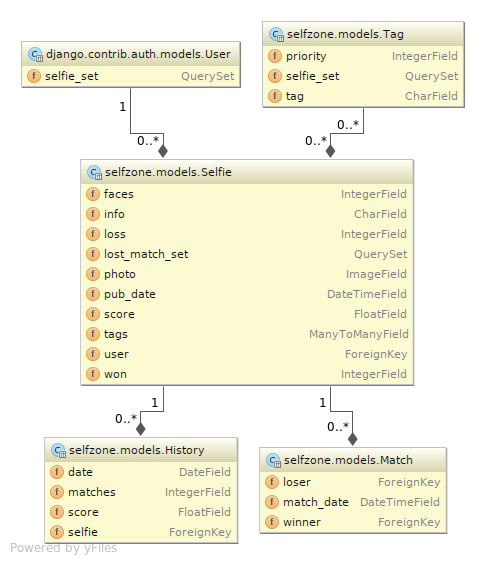
\includegraphics[width=\textwidth]{res/models_diagram.png}
\clearpage

\subsection{User}
Componente del framework Django, contiene i dati degli utenti.

\subsection{Selfie}
La tebella più importante, contiene i dati dei selfie caricati dagli utenti.
\begin{itemize}
\item photo: percoso dell' immagine nel filesystem
\item user: utente che ha caricato il selfie
\item pub\_date: data di caricamento
\item info: descrizione
\item won: numero di sfide vinte dal selfie
\item loss: numero di sfide perse dal selfie
\item score: punteggio del selfie
\item faces: numero di facce presenti nel selfie
\item tags: tags associate al selfie
\end{itemize}

\subsection{Tag}
Contiene le associazioni Tag-Selfie che permettono di discriminare le immagini per parole chiave.
\begin{itemize}
\item tag: parola chiave
\item priority: importanza del tag
\item selfie: selfie associato
\end{itemize}

\subsection{Match}
Tiene conto di ogni sfida a cui anno preso parte i selfie
\begin{itemize}
\item match\_date: data della sfida
\item winner: selfie vincitore
\item loser: selfie perdente
\end{itemize}

\subsection{History}
Per ogni giorno salva gli score parziali di ogni selfie
\begin{itemize}
\item date: giorno
\item score: punteggio parziale
\item selfie: selfie associato
\item matches: sfide a cui ha partecipato
\end{itemize}


\end{document}
